
\section*{Общая характеристика работы}

\newcommand{\actuality}{\underline{\textbf{\actualityTXT}}}
\newcommand{\progress}{\underline{\textbf{\progressTXT}}}
\newcommand{\aim}{\underline{{\textbf\aimTXT}}}
\newcommand{\tasks}{\underline{\textbf{\tasksTXT}}}
\newcommand{\novelty}{\underline{\textbf{\noveltyTXT}}}
\newcommand{\influence}{\underline{\textbf{\influenceTXT}}}
\newcommand{\methods}{\underline{\textbf{\methodsTXT}}}
\newcommand{\defpositions}{\underline{\textbf{\defpositionsTXT}}}
\newcommand{\reliability}{\underline{\textbf{\reliabilityTXT}}}
\newcommand{\probation}{\underline{\textbf{\probationTXT}}}
\newcommand{\contribution}{\underline{\textbf{\contributionTXT}}}
\newcommand{\publications}{\underline{\textbf{\publicationsTXT}}}


{\actuality} Информационная безопасность в современном обществе приобретает все большую актуальность, так как большое количество информации, появление современных гаджетов и развитие технологий привели к становлению постинформационного общества. Данное общество можно характеризовать как  общество потребления большого количества информации, зависимости от информационных и компьютерных технологий, а также как общество с ведущим типом коммуникации – массовой коммуникацией \cite{самойлова2016трансформации}. Человек оказывается в непрерывном удаленном взаимодействии с людьми, юридическими лицами и различным цифровыми инструментами, при этом в течении дня он вынужден многократно проходить процедуры идентификации и аутентификации в различных мобильных приложениях для совершения различных действий, будь то отправка сообщений, чтение почты или совершение платежа. При выполнении этих процедур задействованы самые разнообразные мобильные устройства, а значит задача обеспечения надежной, быстрой и удобной аутентификации в мобильных приложениях является на сегодняшний день крайне актуальной.

% замечания от В.Г. 
% весь общий анализ запихнуть во введение. В первой главе поконкретней.


%Используемые в настоящее время методики аутентификации можно подразделить на четыре категории:
%\begin{enumerate}
%\item Что пользователь знает (пароли и т.д.);
%\item что пользователь имеет (смарт карты, токены и т.д. );
%\item что есть
%\end{enumerate}



Безусловно, среди технологий аутентификации наибольшую привлекательность имеют биометрические методики. Они имеют высокую степень достоверности за счет уникальности биометрических признаков и неотделимости их от дееспособной личности. Однако, использование традиционных биометрических методик для аутентификации порою оказывается не достаточно надежными, в связи с параллельными работами над методиками их взлома \cite{богданов2017обзор}. 

Одним из путей повышение надежности аутентификации является использование комбинированных (мультимодальных) методик, сочетающих в себе технологии идентификации одновременно по нескольким признакам или категориям. Например технологии попадающие одновременно во все три категории аутентификации: <<что человек знает>>, <<что человек имеет>> и <<что есть сам человек>>. Реализация таких методик может предполагать использование дополнительных устройств. Логичнее всего в качестве таких устройств использовать что-то достаточно распространенное. В настоящее время становятся популярными умные устройства, подразумевающие повседневное ношение на запястье и осуществляющие постоянное взаимодействие с человеком - это различные модификации фитнес-браслетов и умных часов. Эти устройства разработаны, в том числе, для контроля биологических параметров и в соответствии с парадигмой интернета вещей представляют собой интерфейс <<Человек-тело-вещь>>. Объем продаж эти устройств в мире составляет десятки миллионов единиц в год.

Использование данного класса устройств совместно с традиционными смартфонами в биометрической аутентификации позволяет повысить информационную безопасность пользователей без необходимости разработки нового оборудования. При этом повышение точности аутентификации будет достигнуто за счет следующих факторов:

\begin{enumerate}
\item Наручное устройство будет являться ключом (токеном) для аутентификации в мобильном устройстве, реализуя проверку, которую можно отнести к категории <<что пользователь имеет>>. В случае кражи любого из устройств доступ злоумышленника к данным пользователя будет закрыт.
\item Наручное устройство, совместно с мобильным, будут задействованы в  аутентификации, использующей жестовую манипуляцию, и, следовательно являющуюся биометрической, относящейся к категории <<что есть сам человек>>. При этом регистрация биометрического признака (в данной работе в качестве него выбран жест) проводится датчиками двух устройств, одновременно контактирующими с разными частями тела человека -  с кистью руки и запястьем, и следовательно, учитывающими большее количество информации о биометрическом признаке по сравнению с аналогичной методикой, использующей только одно устройство. 
\item Аутентификация при помощи двух устройств использующая механизм жестовой манипуляции подразумевает, что пользователь должен знать и уметь выполнить определенный заранее придуманный жест. Следовательно такую аутентификацию можно отнести к категории <<что человек знает>>. 
\end{enumerate}

%Таким образом, задача разработки новых мтодик аутентификации с целью %повышения информационной безопасности, в условиях непрерывного %удаленного взаимодействия людей и цифровых инструментов, является на %сегодняшний день крайне актуальной.

{\aim} данной работы является повышение эффективности биометрической аутентификации при помощи жеста, совершаемого мобильным устройством. 

Для~достижения поставленной цели решались следующие {\tasks}:
\begin{enumerate}
  \item Анализ разработанных методик аутентификации пользователей в мобильных приложениях, выявление их достоинств и недостатков.
  \item Выявление класса задач, повышение эффективности решения которых может быть достигнута с использованием аутентификации при помощи жеста, совершаемого мобильным устройством (далее -- механизма жестовой манипуляции). 
  \item Разработка и исследование методов повышения надежности аутентификации за счет одновременного использования дополнительного устройства.
  \item Разработка комплекса программ аутентификации с помощью жеста.
  \item Проведение экспериментов по применению методики аутентификации для подтверждения полученных результатов, а также получение базы попыток, достаточной для получения приемлемой достоверности результатов при обработке статистических данных и последующего моделирования.
  \item Выбор наиболее эффективного с точки зрения надежности алгоритма реализации методики.
  \item Реализация разработанной методики в виде аппаратно-программного комплекса и проведение его опытной эксплуатации.
\end{enumerate}

\textbf{Объект исследования:} Биометрические системы, использующие для идентификации и аутентификации жесты, совершаемые мобильными устройствами. 

\textbf{Предмет исследования:} Методы аутентификации пользователей мобильных приложений с использующих жесты, совершаемые мобильными устройствами.

{\novelty}
\begin{enumerate}
  \item Методика биометрической аутентификации с помощью жестовой манипуляции, регистрируемая акселерометрами двух взаимодействующими друг с другом устройствами.
  \item Определение порога срабатывания как максимального расстояния от эталона, полученного выполнением серии жестовых манипуляций.
 \item Ранжирование  надежности примененного для аутентификации жеста в зависимости от суммы модулей значений ускорений.  
\end{enumerate}
 

{\influence}: 

\begin{enumerate}
	\item Было выполнено оригинальное исследование по классификации жестов пользователей, выбранных в качестве идентификаторов, на устойчивость к спуфингу.
	\item Проведено исследование, определившее равновероятный уровень ошибок первого и второго рода для девяти алгоритмов, позволившее наглядно доказать эффективность выбранного алгоритма.
	\item Разработаны мобильное приложение и аппаратно-программный комплекс, реализующий разработанную методику. 
\end{enumerate}

Результаты данной работы были результатами научно-исследовательской работы (НИР), проводимой  ФГОБУ <<Финансовый университет>> за 2017 года и признано результатом интеллектуальной деятельности данной НИР. Результаты данной работы были применены в создании аппаратно-программного комплекса АПК <<Замок МТДП>>, опытная эксплуатация которого успешно проводиться на предприятии АО <<НИИЧаспром>>.

{\methods} В ходе исследования применялись методы математической статистики, теории вероятности, теории информации, теории распознавания образов, компьютерного имитационного моделирования. 

Для компьютерного моделирования применялись программы, написанные на языке Matlab. Для реализации комплекта программ применялись языки Java и C.

{\defpositions}
\begin{enumerate}
  \item Использование двух взаимодействующих друг с другом источников регистрации жестовой манипуляции для увеличения надежности системы аутентификации.
  \item Методика суммарной оценки соответствия воспроизведенного жеста эталону.
  \item Методика ранжирования по сумме значений ускорений для классификации надежности жестовой манипуляции. 
\end{enumerate}
%В папке Documents можно ознакомиться в решением совета из Томского ГУ
%в~файле \verb+Def_positions.pdf+, где обоснованно даются рекомендации
%по~формулировкам защищаемых положений. 

{\reliability} полученных результатов подтверждена проведенными экспериментами.

% а так же обоснована и строго доказанных и корректно используемых выводах фундаментальных и прикладных наук, положения которых нашли применение в работе, корректностью постановок задач, применением строгого математического аппарата, отсутствием противоречия между результатами диссертационной работы, сделанными на их основании выводами имитационного и известными компьютерного научными моделирования, фактами, результатами апробацией основных теоретических положений в печатных трудах ВАК и докладах на отечественных и международных научных конференциях. Результаты находятся в соответствии с результатами, полученными другими авторами.

%текс хороший антиплагиат ругается

{\probation}
Основные результаты работы докладывались~на трех Российских и одной международной конференциях.

{\contribution} Автор принимал активное участие в научно-исследовательском процессе Финансового университета. Им был разработан макет для демонстрации возможностей методики, а также образец аппаратно-программного комплекса, реализующий управления запирающим устройством посредством мультимодальной аутентификации пользователя при помощи механизма жестовой манипуляции. 

%\publications\ Основные результаты по теме диссертации изложены в ХХ печатных изданиях~\cite{Sokolov,Gaidaenko,Lermontov,Management},
%Х из которых изданы в журналах, рекомендованных ВАК~\cite{Sokolov,Gaidaenko}, 
%ХХ --- в тезисах докладов~\cite{Lermontov,Management}.

\ifnumequal{\value{bibliosel}}{0}{% Встроенная реализация с загрузкой файла через движок bibtex8
    \publications\ Основные результаты по теме диссертации изложены в XX печатных изданиях,
    X из которых изданы в журналах, рекомендованных ВАК,
    X "--- в тезисах докладов.%
}{% Реализация пакетом biblatex через движок biber
%Сделана отдельная секция, чтобы не отображались в списке цитированных материалов
    \begin{refsection}[vak,wos,scopus,papers,conf]% Подсчет и нумерация авторских работ. Засчитываются только те, которые были прописаны внутри \nocite{}.
        %Чтобы сменить порядок разделов в сгрупированном списке литературы необходимо перетасовать следующие три строчки, а также команды в разделе \newcommand*{\insertbiblioauthorgrouped} в файле biblio/biblatex.tex
        \printbibliography[heading=countauthorvak, env=countauthorvak, keyword=biblioauthorvak, section=1]%
        \printbibliography[heading=countauthorwos,env=countauthorwos, keyword=biblioauthorwos, section=1]%
        \printbibliography[heading=countauthorscopus,env=countauthorscopus, keyword=biblioauthorscopus, section=1]%
	\printbibliography[heading=countauthorconf, env=countauthorconf, keyword=biblioauthorconf, section=1]%
        \printbibliography[heading=countauthorothers, env=countauthorothers, keyword=biblioauthorothers, section=1]%
        \printbibliography[heading=countauthor, env=countauthor, keyword=biblioauthor, section=1]%
        \nocite{%Порядок перечисления в этом блоке определяет порядок вывода в списке публикаций автора
                vakbib1,vakbib2,%
		wosbib1,%
		scbib1,%
                confbib1,confbib2,%
                bib1,bib2,%
        }%
	\publications\ Основные результаты по теме диссертации изложены
	\setcounter{citeauthorscwostot}{\value{citeauthorscopus}} % вместе setcounter и addtocounter добавляют пробел между словами. По-этому они так раскиданы.
        в~\arabic{citeauthor}~печатных изданиях,
	\addtocounter{citeauthorscwostot}{\value{citeauthorwos}}
	\arabic{citeauthorvak} из которых изданы в журналах, рекомендованных ВАК\sloppy
	\ifnum \value{citeauthorscwostot}>0
	, \arabic{citeauthorscwostot} "--- в~периодических научных журналах, индексируемых Web of Science и Scopus\sloppy
	\fi
	\ifnum \value{citeauthorconf}>0
	, \arabic{citeauthorconf} "--- в~тезисах докладов.
	\else
	.
	\fi
    \end{refsection}
    \begin{refsection}[vak,wos,scopus,papers,conf]%Блок, позволяющий отобрать из всех работ автора наиболее значимые, и только их вывести в автореферате, но считать в блоке выше общее число работ
        \printbibliography[heading=countauthorvak, env=countauthorvak, keyword=biblioauthorvak, section=2]%
        \printbibliography[heading=countauthorwos, env=countauthorwos, keyword=biblioauthorwos, section=2]%
        \printbibliography[heading=countauthorscopus, env=countauthorscopus, keyword=biblioauthorscopus, section=2]%
        \printbibliography[heading=countauthorothers, env=countauthorothers, keyword=biblioauthorothers, section=2]%
        \printbibliography[heading=countauthorconf, env=countauthorconf, keyword=biblioauthorconf, section=2]%
        \printbibliography[heading=countauthor, env=countauthor, keyword=biblioauthor, section=2]%
        \nocite{vakbib2}%vak
        \nocite{bib1}%other
        \nocite{confbib1}%conf
    \end{refsection}
}
%При использовании пакета \verb!biblatex! для автоматического подсчёта
%количества публикаций автора по теме диссертации, необходимо
%их~здесь перечислить с использованием команды \verb!\nocite!.
 % Характеристика работы по структуре во введении и в автореферате не отличается (ГОСТ Р 7.0.11, пункты 5.3.1 и 9.2.1), потому её загружаем из одного и того же внешнего файла, предварительно задав форму выделения некоторым параметрам

%Диссертационная работа была выполнена при поддержке грантов ...

%\underline{\textbf{Объем и структура работы.}} Диссертация состоит из~введения, четырех глав, заключения и~приложения. Полный объем диссертации \textbf{ХХХ}~страниц текста с~\textbf{ХХ}~рисунками и~5~таблицами. Список литературы содержит \textbf{ХХX}~наименование.

%\newpage
\section*{Содержание работы}
Во \underline{\textbf{введении}} обосновывается актуальность исследований, проводимых в~рамках данной диссертационной работы, формулируется цель, ставятся задачи работы, излагается научная новизна и практическая значимость представляемой работы.

В~последующих главах сначала описывается сущность проблемы и проводится анализ предметной области. Раскрываются проблемы биометрических и небиометрических методов аутентификации. Проводится выбор алгоритма обработки биометрического признака и логики работы системы аутентификации. Проведен ряд экспериментов, позволивших определить наиболее эффективные решения. На основе полученных решений создан аппаратно-программный комплекс, получивший внедрение на режимном объекте АО <<НИИЧаспром>>.


\underline{\textbf{Первая глава}} посвящена анализу существующих методов аутентификации в мобильных приложениях. Описаны проблемы классической биометрии (отпечаток пальца, речевая аутентификация и аутентификация по биометрическим признакам лица), применяемой в мобильных приложениях \cite{czajka2018presentation} \cite{goicoechea2018attack} \cite{kinnunen2018spoofing}. Раскрыты подходы к разработкам, аутентификации при помощи жестовой манипуляции и приведены существующие недостатки этих методов.

В заключительной части первой главы сформулирована задача создания мультимодальной аутентификация пользователей мобильных приложений с использованием жестовой манипуляции, позволяющая преодолеть многие из них за счет одновременного использования для аутентификации трех факторов - <<Что пользователь знает>>, <<Что пользователь имеет>> и <<Что есть сам пользователь>> (биометрический фактор).

Суть данной методики в использовании двух взаимоувязанных устройств. На рисунке \ref{img:guest1} представлен пример аутентификации.
\begin{figure}[ht] 
	\centering
	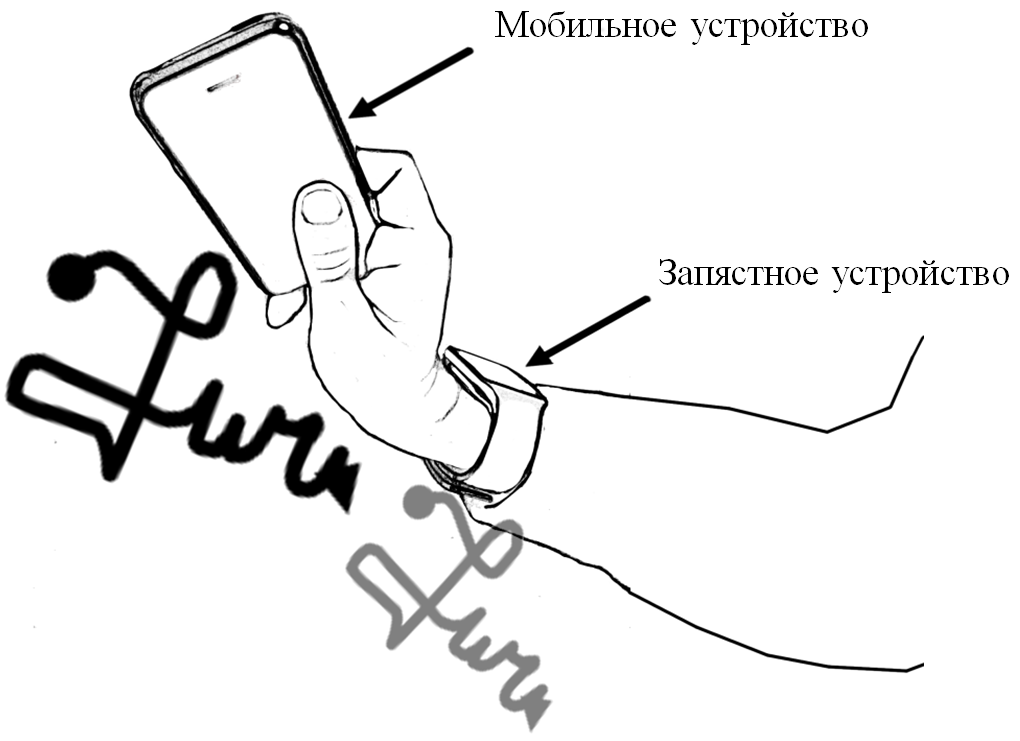
\includegraphics [scale=0.25] {guest}
	\caption {Пример использования аутентификации пользователей мобильных приложений с использованием жестовой манипуляции}
	\label{img:guest1}
\end{figure}

Жест, который был выбран пользователем в качестве аутентифицирующего, необходимо запомнить, чтобы впоследствии воспроизводить его с достаточной точностью. Для запоминания жеста необходимо некоторое время его тренировать. Функция тренировки жеста была реализована в макете и подтвердила свою функциональность.   

Работа по исследованию алгоритмов аутентификации при помощи жестовой манипуляции опирается на труды сотрудников Университета Райса - Jiayang Liua и Lin Zhonga, а также сотрудников фирмы Мотролла - Jehan Wickramasuriyab и Venu Vasudevanb, которые в 2008 - 2009 году впервые предложили  аутентификацию при помощи жестовой манипуляции (манипуляции джойстиком устройства) \cite{liu2009uwave, liu2009user}.

\underline{\textbf{Вторая глава}} посвящена исследованием путей реализации методики в приложениях. В первом разделе второй главы проведен анализ пространства биометрических признаков жестовой манипуляции и формализована задача определения соответствия биометрического признака эталону.  

Проведено описание алгоритмов, способных выполнять задачи сравнения биометрического признака  эталоном. Рассмотрено несколько вариантов логики получения биометрического признака и способы классификации его надежности.  Определен доверительный интервал оценки ошибок первого и второго рода в соответствии с формулой~\ref{eq:dvin} \cite[с.~46]{MatStat_1960}: % страничка проверена

\begin{equation}
\label{eq:dvin}
p=\frac{n}{g^{2}+n} \left (\omega +\frac{g^2}{2\cdot n}\pm g\cdot \sqrt{\frac{\omega \cdot (1-\omega)}{n}+ \frac{g^2}{4\cdot n^2}} \right ),
\end{equation}

С учетом количества экспериментов не менее $n = 1000$ для определения ошибок первого рода и $n = 4000 $ для определения ошибок второго он определен как $p_{1}\in\left[ 0,016;0,036   \right]$, $p_{2}\in\left[ 0,02;0,03 \right]$.

\underline{\textbf{Третья глава}} посвящена исследованию алгоритмов обработки биометрических признаков жестовой манипуляции. Приведены результаты эксперимента, на основе которых с помощью компьютерного моделирования был проведен поиск комплексного критерия качества для девяти алгоритмов, показавший, что наиболее эффективными являются алгоритмы основанные на динамическом сдвиге шкалы времени (DTW). 

В качестве критерия качества был выбран равный уровень ошибок первого и второго рода EER (equal error rate).

Лучшие результаты получены в случае использования для обработки биометрического признака алгоритмом DTW, в котором для построения матрицы расстояний применяется расстояние Евклида.

Визуализация результатов моделирования и график зависимости ошибок первого и второго рода от значения порога для DTW представлены на рисунке \ref{img:sil-dtw-ev}.     

\begin{figure}[ht] 
	\centering
	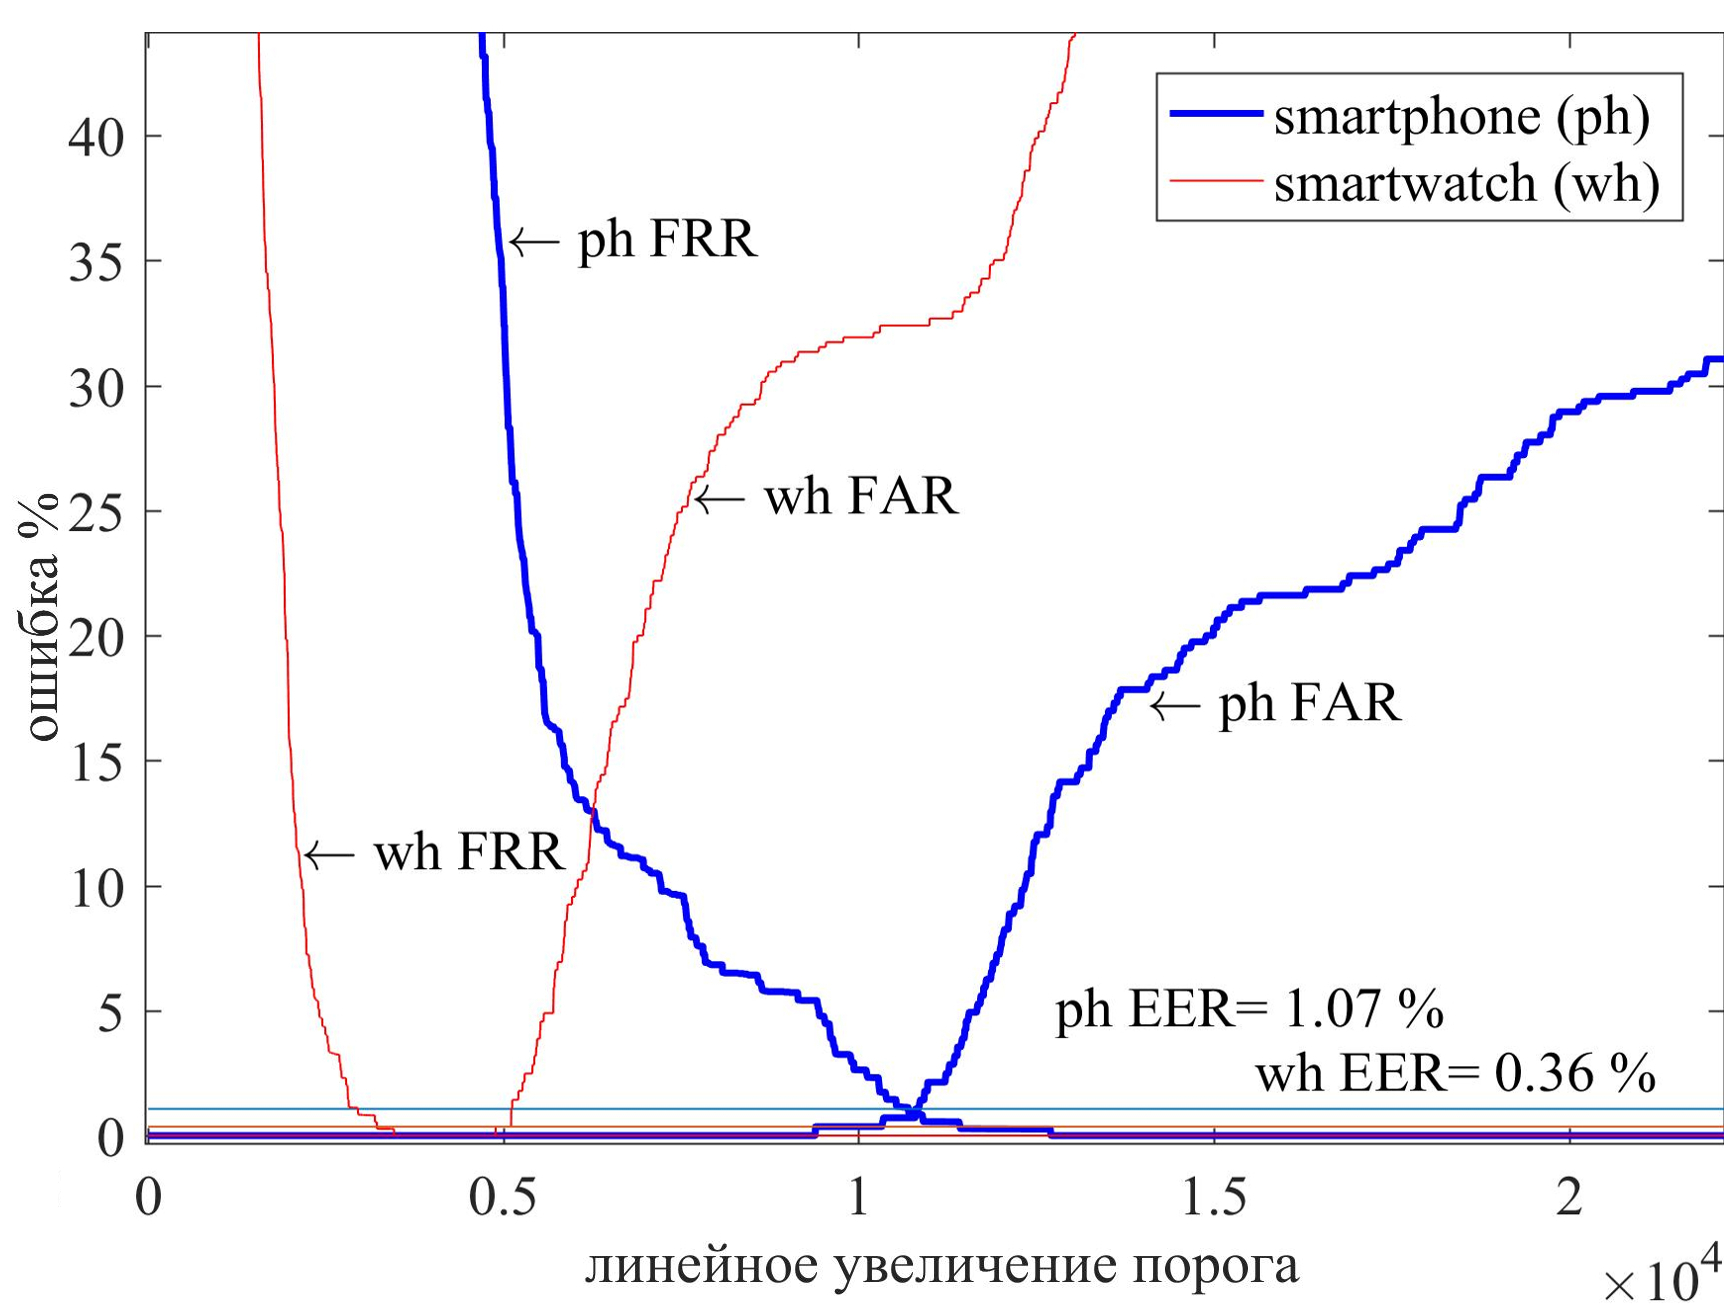
\includegraphics [width=7.5cm] {sil-dtw-ev} %
	\caption {Ошибки  первого рода - FRR, второго рода - FAR, и EER для умных часов (красные графики) и смартфона (синие графики). Алгоритм DTW, использующий для построения матрицы расстояний расстояние Евклида}
	\label{img:sil-dtw-ev}
\end{figure}

Моделирование включало имитацию $2 \cdot 10^4$ попыток аутентификации для каждого алгоритма. 

При использовании DTW интенсивные жесты, классифицированные как надежные, имеют значение EER для биометрической составляющей менее 0.36~\%, что имеет достаточную надежность при эксплуатации системы аутентификации в реальных условиях.  
%Можно сослаться на свои работы в автореферате. Для этого в файле
%\verb!Synopsis/setup.tex! необходимо присвоить положительное значение
%счётчику \verb!\setcounter{usefootcite}{1}!. В таком случае ссылки на
%работы других авторов будут подстрочными.
%\ifnumgreater{\value{usefootcite}}{0}{
%Изложенные в третьей главе результаты опубликованы в~\cite{vakbib1, vakbib2}.
%}{}
%Использование подстрочных ссылок внутри таблиц может вызывать проблемы.

В \underline{\textbf{четвертой главе}} приведено описание различных применений методов  мультимодальной аутентификации пользователей мобильных приложений с использованием механизма жестовой манипуляции в реальных условиях применительно к аппаратно-программным комплексам.

Глава включает в себя проработку вопроса безопасности мобильного приложения с точки зрения информационной безопасности, как при клиент-серверной архитектуре аутентификации, так и при использовании автономного мобильного приложения. 

Глава описывает функциональную схему аппаратно-программного комплекса (АПК) <<Замок-МТДП>>, описаны преимущества и недостатки применения электронных дистанционных систем запирания и для помещений и при использовании в составе несгораемых шкафов и сейфов.  

В конце главы приведен опыт внедрения АПК <<Замок МТДП>> на предприятии АО <<НИИЧаспром>>.

В \underline{\textbf{заключении}} приведены основные результаты работы, которые заключаются в следующем:
%% Согласно ГОСТ Р 7.0.11-2011:
%% 5.3.3 В заключении диссертации излагают итоги выполненного исследования, рекомендации, перспективы дальнейшей разработки темы.
%% 9.2.3 В заключении автореферата диссертации излагают итоги данного исследования, рекомендации и перспективы дальнейшей разработки темы.
\begin{enumerate}
  \item На основе анализа механизмов жестовой манипуляции была разработана концепция методики мультимодальной биометрической аутентификации с использованием двух независимых мобильных устройств - смартфона и умных часов. 
  \item Создан макет для умных часов и смартфона, реализующий аутентификацию, а также сохраняющей данные аутентификации в виде массива временных рядов.
  \item Макет был опробован и доработан в рамках научно-исследовательских работ <<Финансового Университета>> и поставлен на баланс как результат интеллектуальной деятельности Университета. 
  \item При участи группы людей, с использованием макета, была создана база данных попыток аутентификации, составляющая более тысячи попыток.
  \item С использованием базы данных попыток аутентификации было проведено моделирование, определившее уровни равновероятного соотношения ошибок первого и второго уровня (комплексные показатели качества) для различных алгоритмов и определен наиболее удовлетворяющий с точки зрения надежности - алгоритм динамической трансформации шкалы времени с использование алгоритма Евклида для формирования матрицы расстояния.
  \item С применением выбранного алгоритма реализован аппаратно-программный комплекс <<Замок-МТДП>> - осуществляющий  аутентификацию и открытие замка при помощи механизма жестовой манипуляции применяемого для помещений или сейфовых хранилищ предприятия. 
  \item Аппаратно-программный комплекс применен для хранения материальных ценностей на предприятии АО <<НИИЧаспром>> и прошел успешную опытную эксплуатацию. Применение АПК <<Замок-МТДП>> позволило повысить надежность хранения ценностей. 
\end{enumerate}

Полученные результаты позволяют говорить об отработанности методики, и готовности внедрение ее в те сферы обеспечения информационной безопасности, где необходимо проводить срытую и надежную аутентификацию - например аутентификацию в мобильных приложениях, предполагающих работу в людных местах. 

Вторым направлением применения методики могут стать биометрические замки для различных сфер применения со сниженным уровнем энергопотребления.   


%\newpage
%При использовании пакета \verb!biblatex! список публикаций автора по теме
%диссертации формируется в разделе <<\publications>>\ файла
%\verb!../common/characteristic.tex!  при помощи команды \verb!\nocite! 

\ifdefmacro{\microtypesetup}{\microtypesetup{protrusion=false}}{} % не рекомендуется применять пакет микротипографики к автоматически генерируемому списку литературы
\ifnumequal{\value{bibliosel}}{0}{% Встроенная реализация с загрузкой файла через движок bibtex8
  \renewcommand{\bibname}{\large \authorbibtitle}
  \nocite{*}
  \insertbiblioauthor           % Подключаем Bib-базы
  %\insertbiblioother   % !!! bibtex не умеет работать с несколькими библиографиями !!!
}{% Реализация пакетом biblatex через движок biber
  \ifnumgreater{\value{usefootcite}}{0}{
%  \nocite{*} % Невидимая цитата всех работ, позволит вывести все работы автора
  \insertbiblioauthorcited      % Вывод процитированных в автореферате работ автора
  }{
  \insertbiblioauthor           % Вывод всех работ автора
%  \insertbiblioauthorgrouped    % Вывод всех работ автора, сгруппированных по источникам
%  \insertbiblioauthorimportant  % Вывод наиболее значимых работ автора (определяется в файле characteristic во второй section)
  \insertbiblioother            % Вывод списка литературы, на которую ссылались в тексте автореферата
  }
}
\ifdefmacro{\microtypesetup}{\microtypesetup{protrusion=true}}{}

